\section{Proposed Research}
\label{sec:proposed-work}
%The proposed research develops fast,
%high-order-accurate, parallel numerical algorithms for large-scale
%simulations of the collective hydrodynamics of amphiphilic particles in a viscous solvent.
%%
We have demonstrated that our hydrophobic attraction with repulsion potential (HARP) approach efficiently simulates
self-assembly of amphiphilic particles into two-dimensional micelles, bilayer membranes, and vesicles \cite{Fu2018_SIAM}, and
recreates the tank-treading phenomenon in external shear flows
\cite{Fu20}.
%\todo[inline]{!!let's put a proceedings here so we have something to cite!!}.
%
While the results show great promise in the field of collective body hydrodynamics,
several outstanding issues need to be addressed. These include a thorough 
analysis of elastic properties of our coarse-grained bilayers, and 
efficiently simulating three-dimensional collective hydrodynamics of amphiphilic particles.
Finally, we must mathematically characterize the variational behavior of HARP under appropriate homogenized limits.

\subsection{Specific Aim 1: Measuring material properties of self-assembly of amphiphiles}
\label{subsec:specific_aim_1}

%\begin{figure}
%\begin{center}
%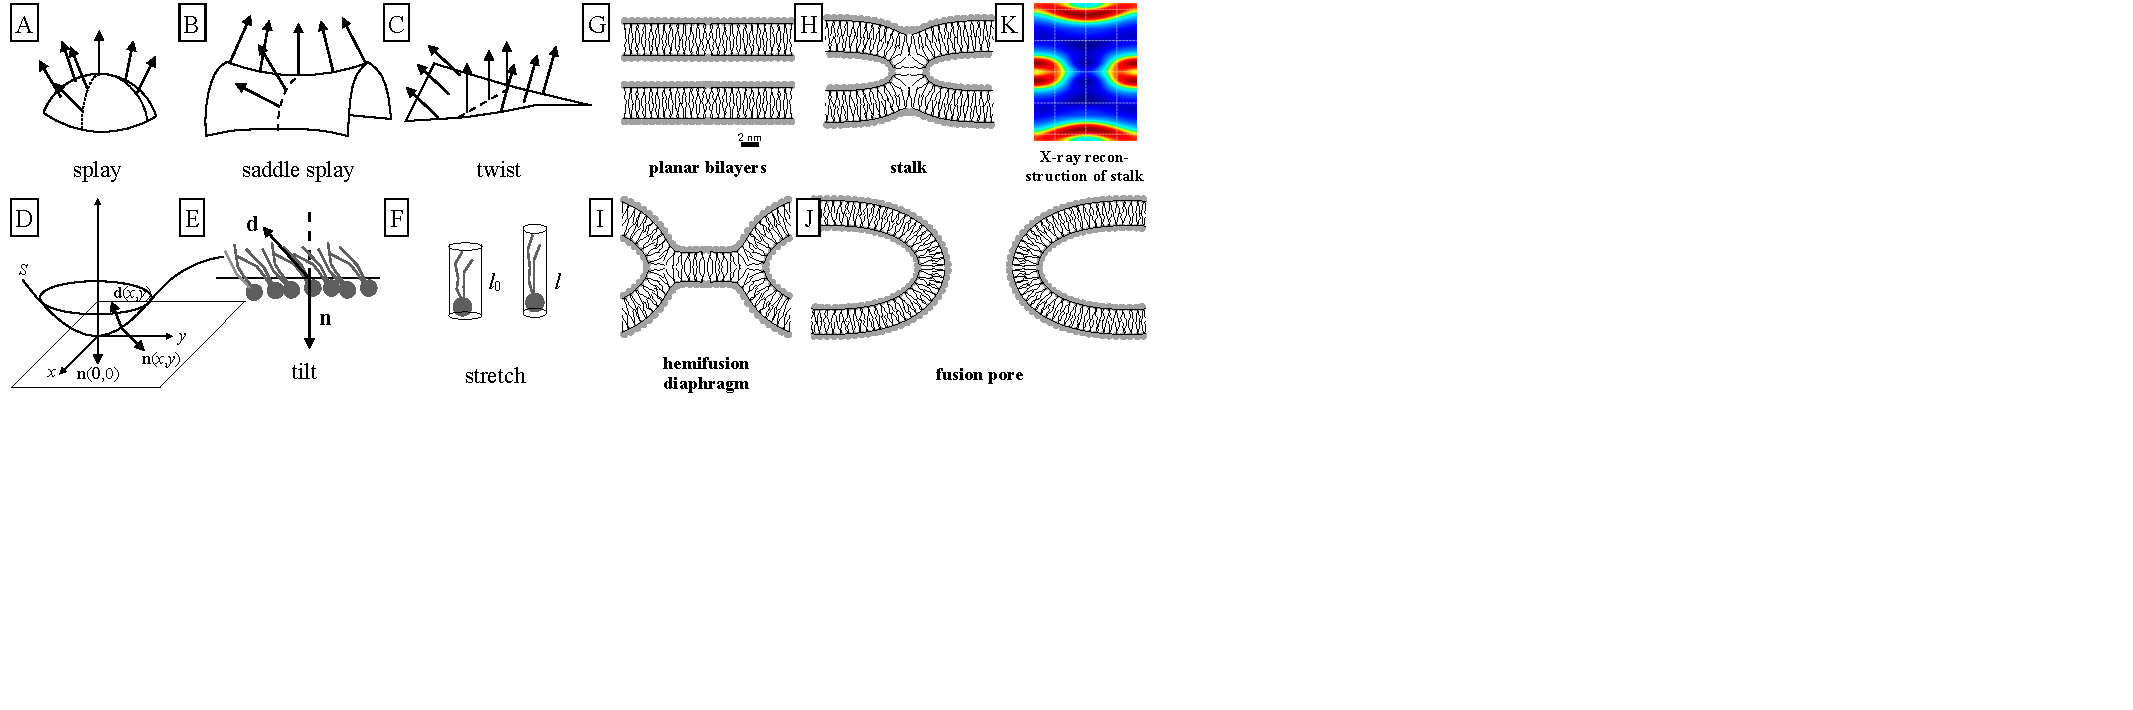
\includegraphics[width=0.9\textwidth]{figures/SA1_fig1.pdf}
%\end{center}
%\caption{\footnotesize (A--C) The splay ($\Div \mathbf{d}$), 
%saddle splay ($\det \mathsf{D}$) and twist ($\Curl \mathbf{d}$) elastic distortions of 
%a monolayer. (D) The monolayer neutral surface $\Sigma$,  
%director $\mathbf{d}$ and unit normal $\mathbf{n}$ in local coordinates.
%(E--F) Lipids are able to tilt from  the surface normal, and stretch.
%(H--J) Intermediates of membrane fusion and (K) experimental image of a stalk \cite{Aeffner2012}. }
%\label{fig:distortions}
%\end{figure}
The goal of Specific Aim 1 is to characterize the material properties of many-body, self-assembled amphiphiles.
For amphiphiles assembled into bilayers, these properties are described by membrane continuum mechanics.
Our goal is to be able to map the parameters of the particle-based model onto the elastic moduli from continuum theory.
Results from this goal will facilitate simulators to use the hydrophobic attraction force calculations
to model bilayers with specific composition. These calculations have provably less computational complexity than
those of molecular dynamics simulations and possess the molecular granularity lacking from continuum models.

Hamm and Kozlov (HK) pioneered 
the modern theory of membrane continuum mechanics \cite{Hamm2000}, and their theory
%was pioneered by Hamm and Kozlov (HK) \cite{Hamm2000}. The theory 
is widely used to describe biological phenomona 
fission \cite{FrEsAkSh15, Maetal15, PhysRevE.79.031926},
fusion \cite{ChKo08, KoKo2002,Kuzmin7235,Aeffner2012},
poration \cite{Gaetal20}, phase boundaries and interaction with inclusions
\cite{SeLeMaEg17,Saetal20, Pietal20}, which require resolution of the internal structure of the membrane.  
Recently, there has been a revival in interest in the HK theory as the quadratic assumption
for the elasticity energy density has caused
%Using the HK  model as a base,
%PI RR and collaborators calculated, for the first time in continuum theory, a least energy path for transitions between planar bilayers, a membrane stalk,
%hemifusion diaphragm and the fusion pore \cite{RyWaCo13,RyKlYaCo16},
%and the energies calculated by these continuum studies (Figure \ref{fig:barriers}A),
%are in agreement with barrier heights derived by molecular dynamics and experimental studies \cite{FrRoPi17}.  
%
\begin{wrapfigure}[12]{l}{0.47\textwidth}
\centerline{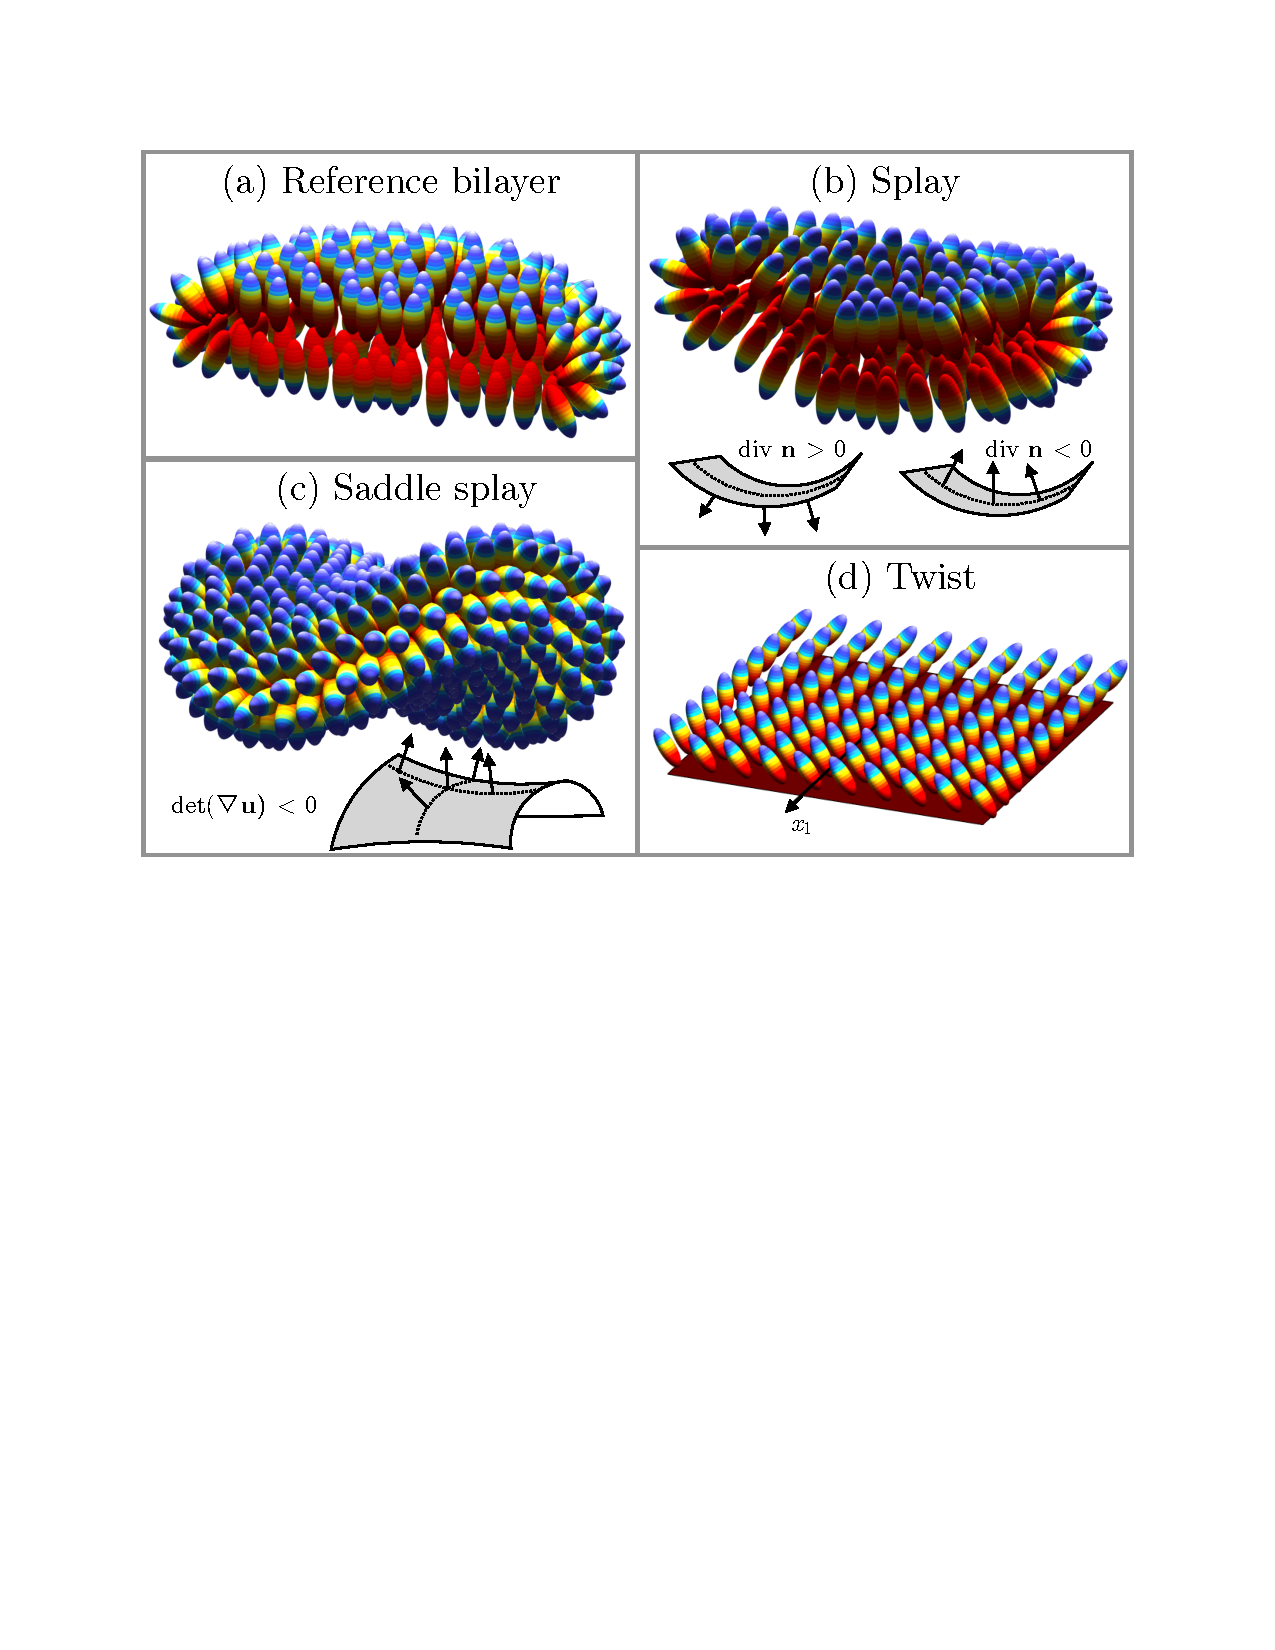
\includegraphics[width=0.47\textwidth]{Figures/Deformations.pdf}}
%  \centering{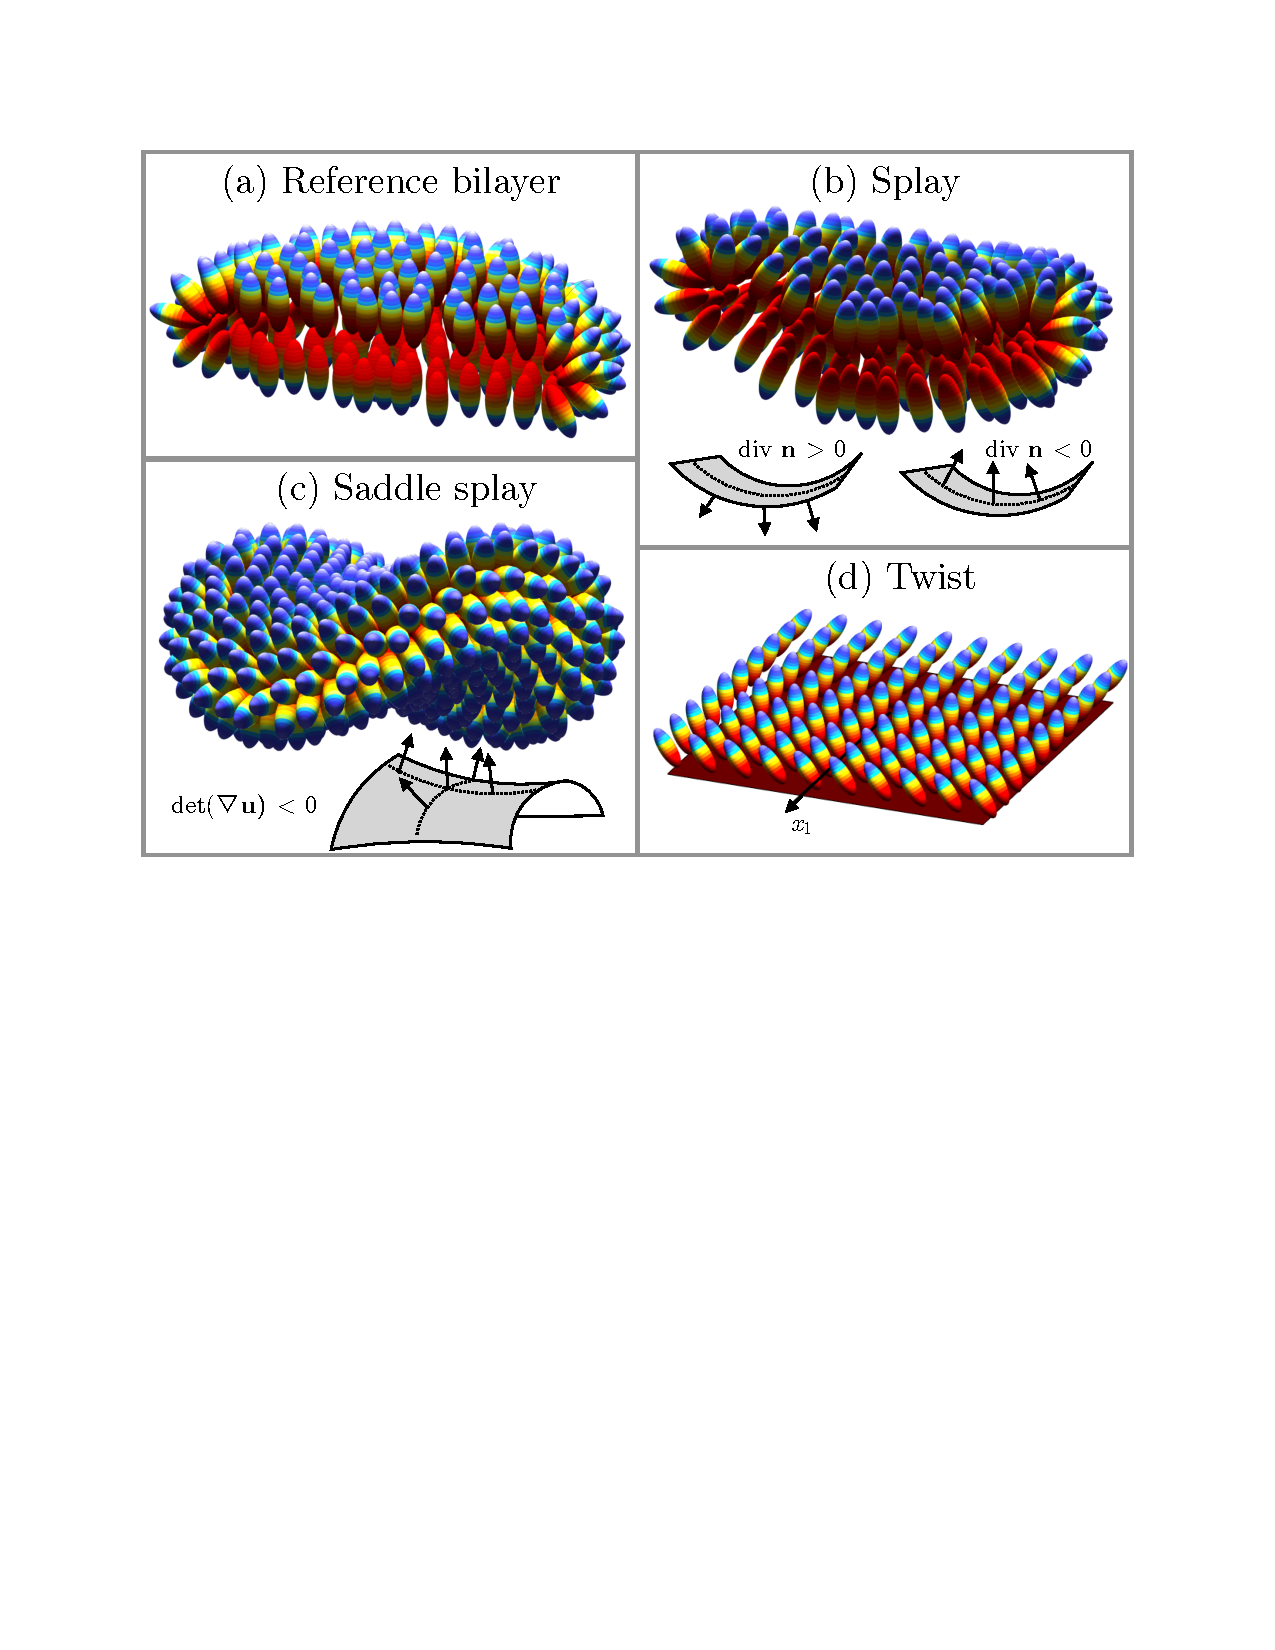
\includegraphics[width=0.80\textwidth]{Figures/Deformations.pdf}}
\caption{\label{fig:deformations}Sketch of the HK membrane model \cite{Hamm2000}.
    }
\end{wrapfigure}
%
 researchers to question the applicability of \eqref{ansatz3} for large curvatures \cite{PhysRevLett.117.188102, ARGUDO20161619}. 
For example, Galimzyanov {\it et al.} \cite{C9SM02079A} countered that energies derived from molecular dynamics and elasticity agree, even when curvatures are large.
This proposal will develop much-needed mathematical analysis to resolve these controversies due to the assumptions in the HK theory. 

%\begin{wrapfigure}[13]{l}{0.5\textwidth}
%\centerline{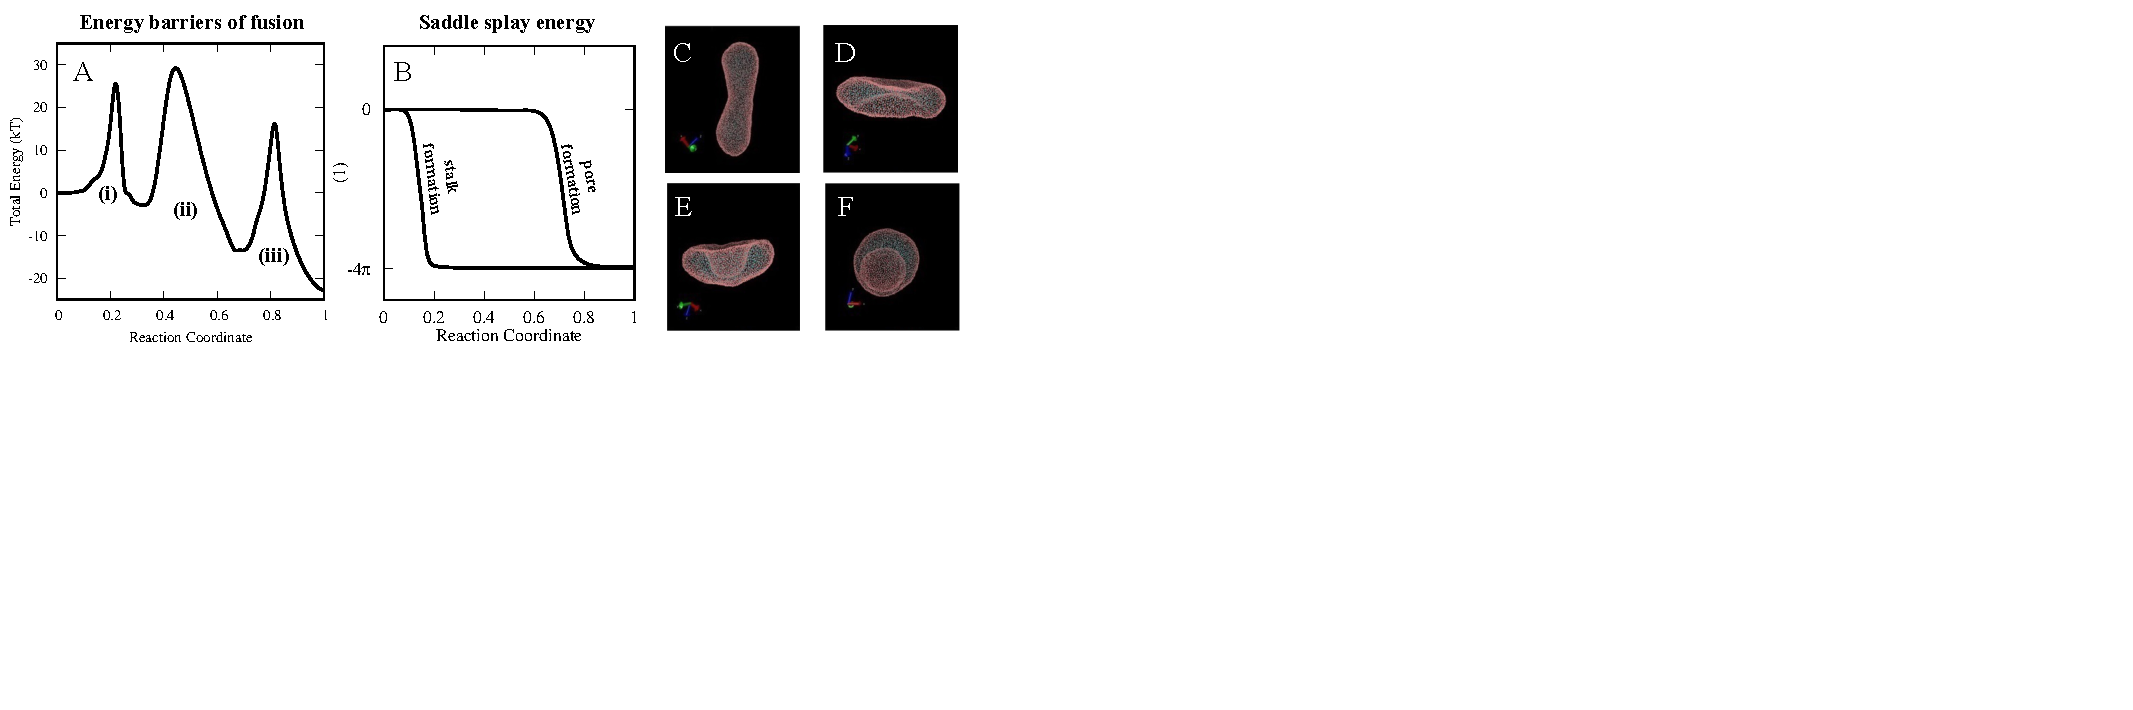
\includegraphics[width=0.5\textwidth]{figures/SA1_fig3.pdf}}
%\caption{{\footnotesize (A) Energy barriers for stalk formation (i), hemifusion
%diaphragm expansion (ii) and pore formation (iii). 
%(B) Saddle-splay energy for each change in \emph{monolayer} topology
%calculated in \cite{RyKlYaCo16}. (C)--(F): Shape transition of vesicle at different values of volume to area ratio from coarse-grained simulations of lipid bilayer membranes \cite{Fu16}.}}
%\label{fig:barriers}
%\end{wrapfigure}

The HK framework assumes a three-dimensional lipid monolayers with internal structure
consisting of straight fibers that represent elongated hydrocarbon chains. HK assumed an
elastic energy density ${\cal W}$ that quadratic in the Green-Lagrange strain tensor for membrane deformation of
this striated, internal structure.
%
%
%
%These fibers
%tilt and stretch with respect to the dividing surface--the surface formed lying between the hydrocarbon chains and polar heads of lipids.
%Accordingly, the deformation takes the form 
%\begin{equation}
%  \label{LMdeformation}
%{\bf x}(X_1, X_2, X_3) = {\bf x}_0(X_1, X_2) + \zeta(x_0(X_1, X_2), X_3) {\bf n}(x_0(X_1, X_2))
%\end{equation}
%where $(X_1,X_2,X_3)$ are points in a reference volume.
%The map $x_0$ parametrizes the dividing surface $\Sigma$, and the unit vector field ${\bf n}$ parametrizes the
%direction of the lipid tails in the deformed state \cite{doi:10.1021/jp075641w,KLAUDA20083074}.
%The parameter $X_3$ and the function $\zeta$ parametrizes the distance along the hydrocarbon chain in the reference state
%and the deformed state, respectively, and so $0 \leq X_3 \leq \delta$ where $\delta = $ 2.5 nm is a realistic monolayer thickness. 
%
%The elastic theory assumes an energy density that is quadratic in the Green-Lagrange strain tensor for ${\bf x}$. 
%The chains stretch and compress to satisfy incompressibility.
%Symmetries with respect to mirror reflection and in-plane rotation, the internal structure assumptions and incompressibility
%lead to an elastic surface energy over the dividing surface $\Sigma$. 
%
This energy decomposes into four, fundamental and independent deformations  (figure~\ref{fig:deformations}):
splay ($\Div {\bf n}$), twist ($\Curl {\bf n}$), saddle splay ($\det \nabla {\bf n}$) and tilt ${\bf t}={\bf n}/({\bf N}\cdot {\bf n}) - {\bf N}$ where ${\bf N}$ is the unit surface normal:
\begin{equation}
\label{ansatz3}
\begin{aligned}
{\cal W} \equiv \int_{\Sigma} 
  \tfrac{1}{2}\KB\left[ \left( \Div {\bf n} + k_0\right)^2 - k_0^2\right] 
+ \tfrac{1}{2}\KT (\Curl {\bf n})^2 + \KG  \det \nabla {\bf n} + \tfrac{1}{2}\KTH |{\bf t}|^2 \,dA.
\end{aligned}
\end{equation}
Here, 
%$(\nabla {\bf n})_{ij} = \partial_{x_j}{\bf n} \cdot {\bf e}_i$ is the surface gradient with
%orthonormal tangent vectors $\{{\bf e}_1, {\bf e}_2\}$.
%%\todo[inline]{YNY and BQ: What do you call a coordinate system where the metric is the identity at one point?}
%Also, the surface divergence 
%$\Div {\bf n}$ is the trace, and the surface curl $\Curl {\bf n}$ is the anti-trace (sum of the off-diagonal elements), of $\nabla {\bf n}$ respectively.
%respectively (Figure \ref{fig:distortions}A--C).
the deformations come with elastic coefficients: the bending modulus $\KB$, twist modulus $\KT$ 
and saddle-splay modulus $\KG$ and tilt modulus $\KTH$
%HK define the tilt vector ${\bf t} = {\bf n}/({\bf N}\cdot {\bf n}) - {\bf N}$ where ${\bf N}$ is the unit surface normal.
%
The parameter $k_0$ is the  spontaneous curvature and it determines the preferred lipid splay \cite{RoLi15,Kozlov2007}. 
As an illustration, the lipid DSPC has $k_0 = -0.1$ nm$^{-1}$ 
%as a result of  %having a relatively long acyl chain. 
and these lipids would line the  inner monolayer of a 
spherical liposome, because the addition of a positive splay $\Div \mathbf{n}$  in \eqref{ansatz3}
to the negative spontaneous curvature $k_0$ leads to lower energy \cite{Kamal22245, C3SM51829A, RoLi15,FriedSeguin15}.
The subtraction of $k_0^2$ makes the energy distortion free
\cite{Helfrich73,PhysRevLett.113.248102,Hamm2000}.

Under spatial scales much larger than the
membrane thickness, membrane energy is well-characterized by the
Canham-Helfrich energy used throughout the fluid-structure literature
\cite{QiangDu09, Lowengrub07,KimLai2010_JCP, Hu, HuLaiSeolEtAl2016_JCP,
  qua-bir2014, qua-vee-you2019}.
%\todo[inline]{YNY: place your recent works here}
The Canham-Helfrich energy is actually a special case of
\eqref{ansatz3} obtained by setting ${\bf n} =  \pm {\bf N}$ (the $\pm$ depending on
orientation) and collapsing both monolayers onto the membrane midplane.
%There, splay $\Div n$ equal to twice the mean curvature, saddle splay
%$\det \nabla n$ equal to the Gauss curvature, and both twist and tilt
%are equal to zero. 

%\begin{figure}
%\begin{center}
%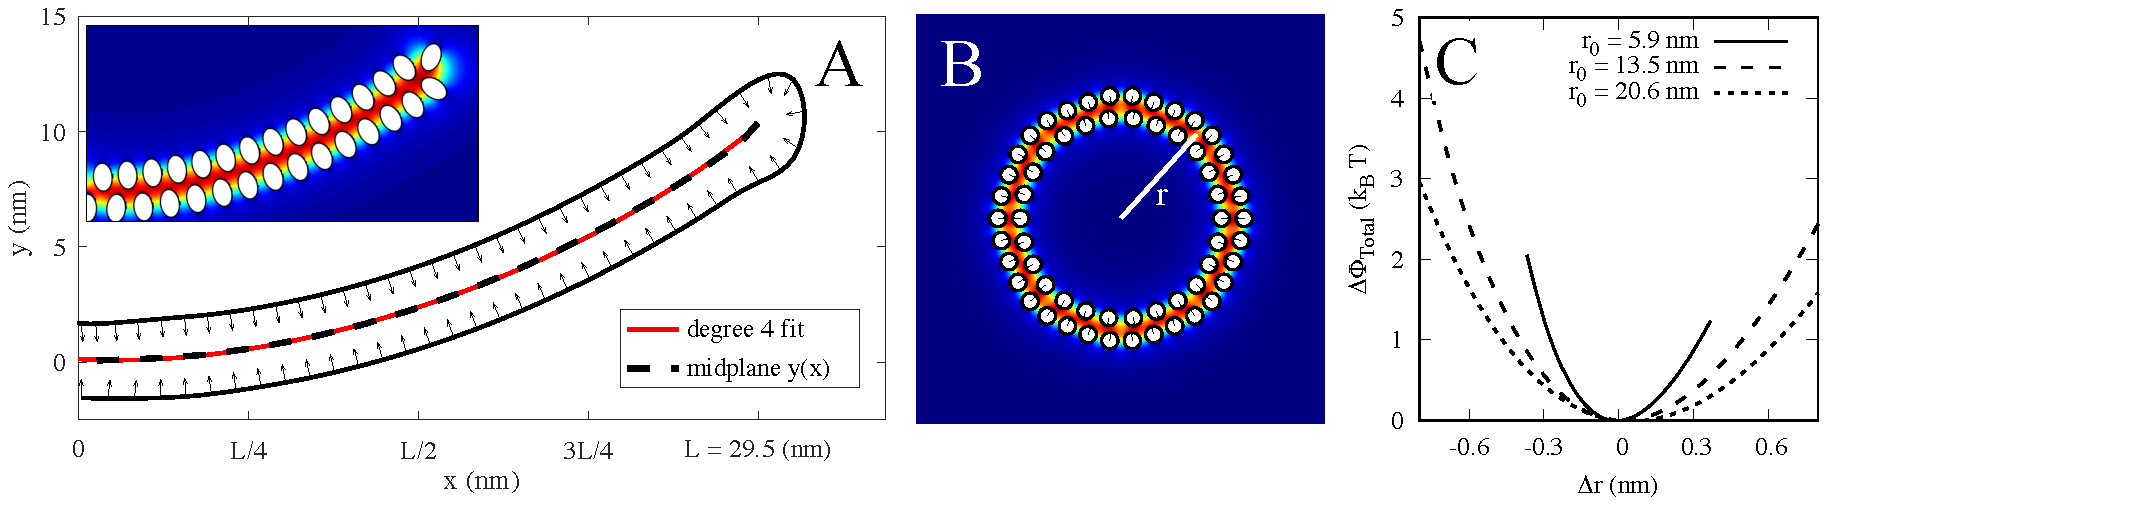
\includegraphics[width=\textwidth]{figures/SA1_fig2.pdf}
%\end{center}\vspace{-1.em}
%\caption{\footnotesize (A) A partially clamped bilayer with mid-plane (dashed curve) under uniform load.
%The quartic fit comes from continuum theory. 
%(B) A circular vesicle at equilibrium. (C) The area modulus derives
%from convexity in energy as a function of radius. 
%\label{fig:bend}}
%\end{figure}


% Proposers should address what they want to do,
% why they want to do it,
% how they plan to do it,
% how they will know if they succeed,
% and what benefits could accrue if the project is successful.
%\begin{center}
%Preliminary results
%\end{center}

%\begin{wrapfigure}[13]{l}{0.5\textwidth}
%\centerline{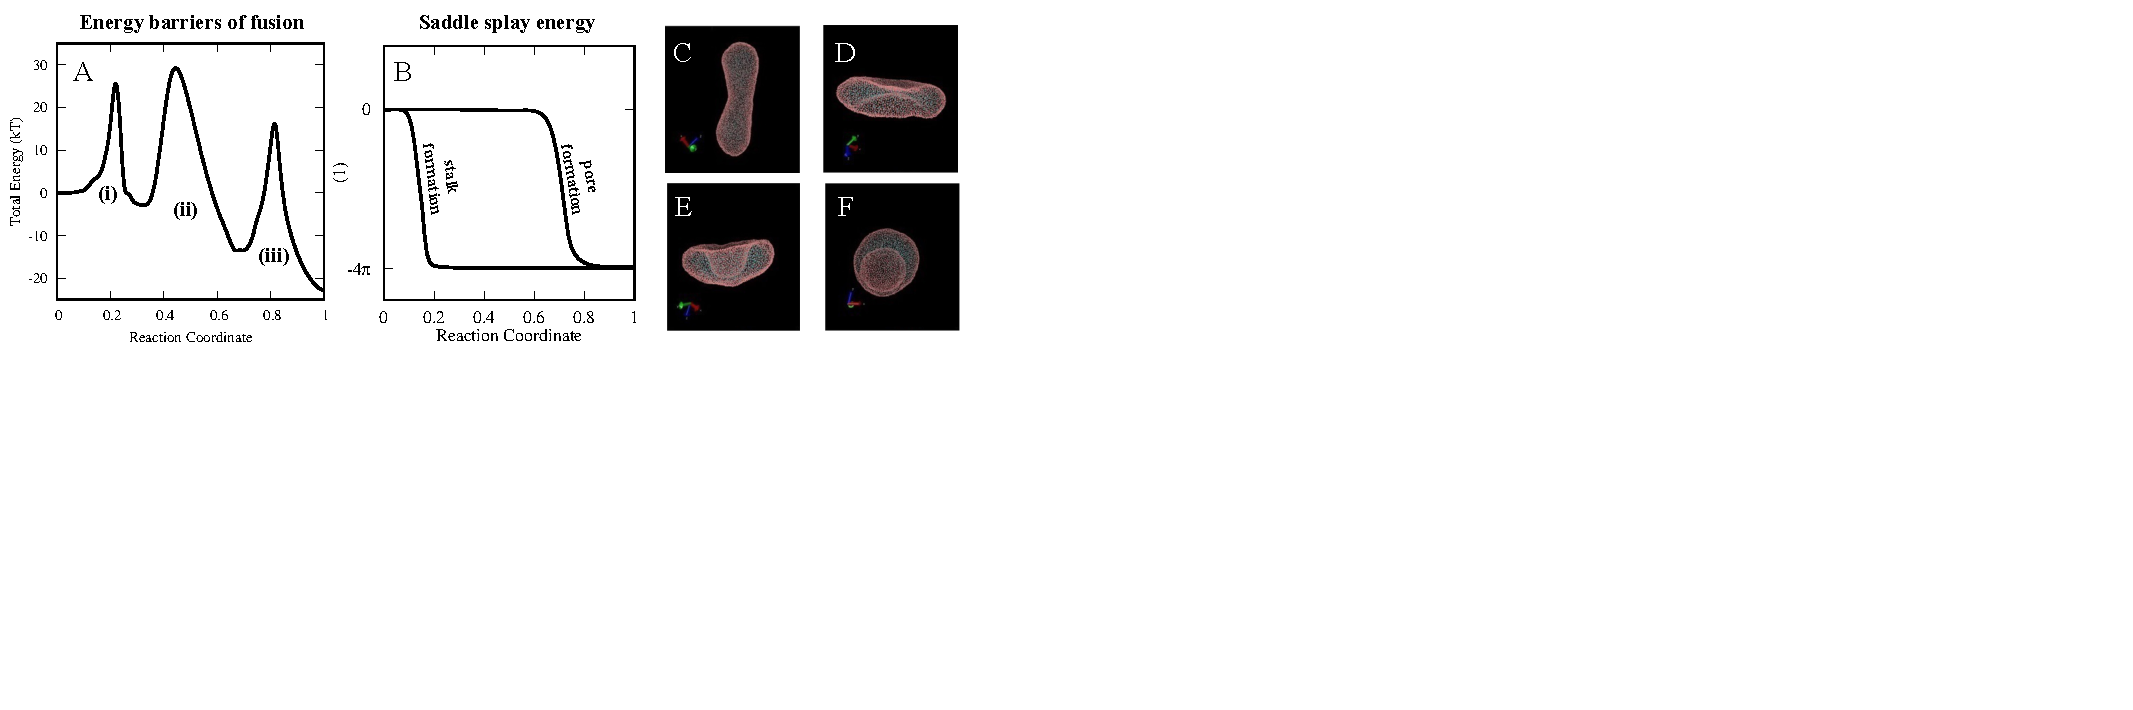
\includegraphics[width=0.5\textwidth]{figures/SA1_fig3.pdf}}
%\caption{{\footnotesize (A) Energy barriers for stalk formation (i), hemifusion
%diaphragm expansion (ii) and pore formation (iii). 
%(B) Saddle-splay energy for each change in \emph{monolayer} topology
%calculated in \cite{RyKlYaCo16}. (C)--(F): Shape transition of vesicle at different values of volume to area ratio from coarse-grained simulations of lipid bilayer membranes \cite{Fu16}.}}
%\label{fig:barriers}
%\end{wrapfigure}

%\begin{center}
%Anticipated model simulations
%\end{center}
\subsubsection{Simulations of the HARP model to estimate elastic moduli}
%To characterize material properties of a bilayer, we compare the energies and forces generated by
%a collection of amphiphilic particles against the energies and forces of a continuum bilayer.
We propose to
%
%to examine conduct calculations similar to the example of figure~\ref{fig:flattening}
%for a wide range of particle parameters and physical parameters in HARP to 
%
%{\bf (i)} Assess whether the continuum energies \eqref{ansatz3} are the same
%as the corresponding energies in the particle system for all reasonable deformation.
%If this is the case we will 
%
{\bf (i)} determine the value of the elastic moduli $\KB$,
$\KT$, $\KG$ and $\KTH$, and then {\bf (ii)} understand how the model parameters $\rho,$ $\gamma$, and particle shape map onto elastic moduli. 
An accurate and robust way to measure material properties is to track the evolution of the bilayer as
%
\begin{wrapfigure}[10]{r}{0.4\textwidth}
\vspace{-0.3cm}
\centerline{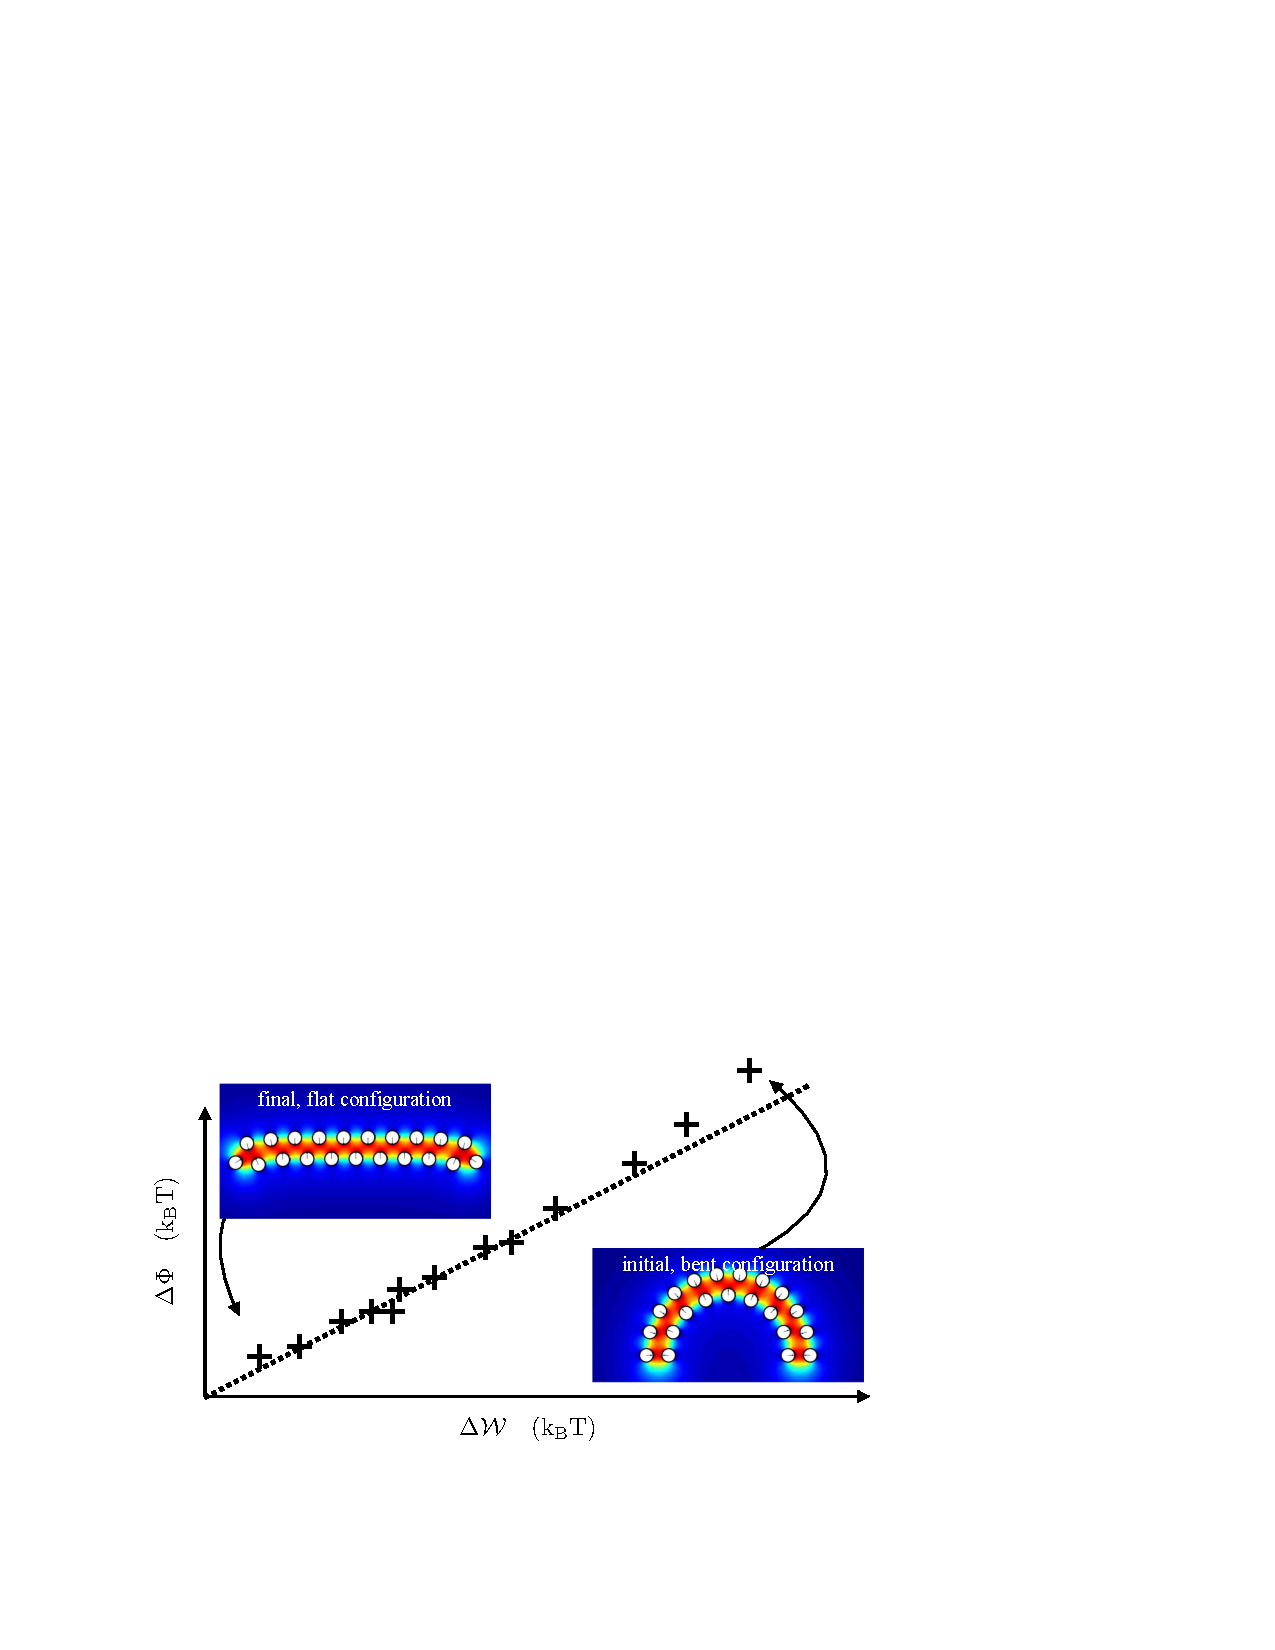
\includegraphics[width=0.4\textwidth]{Figures/Flattening.pdf}}
%  \centering{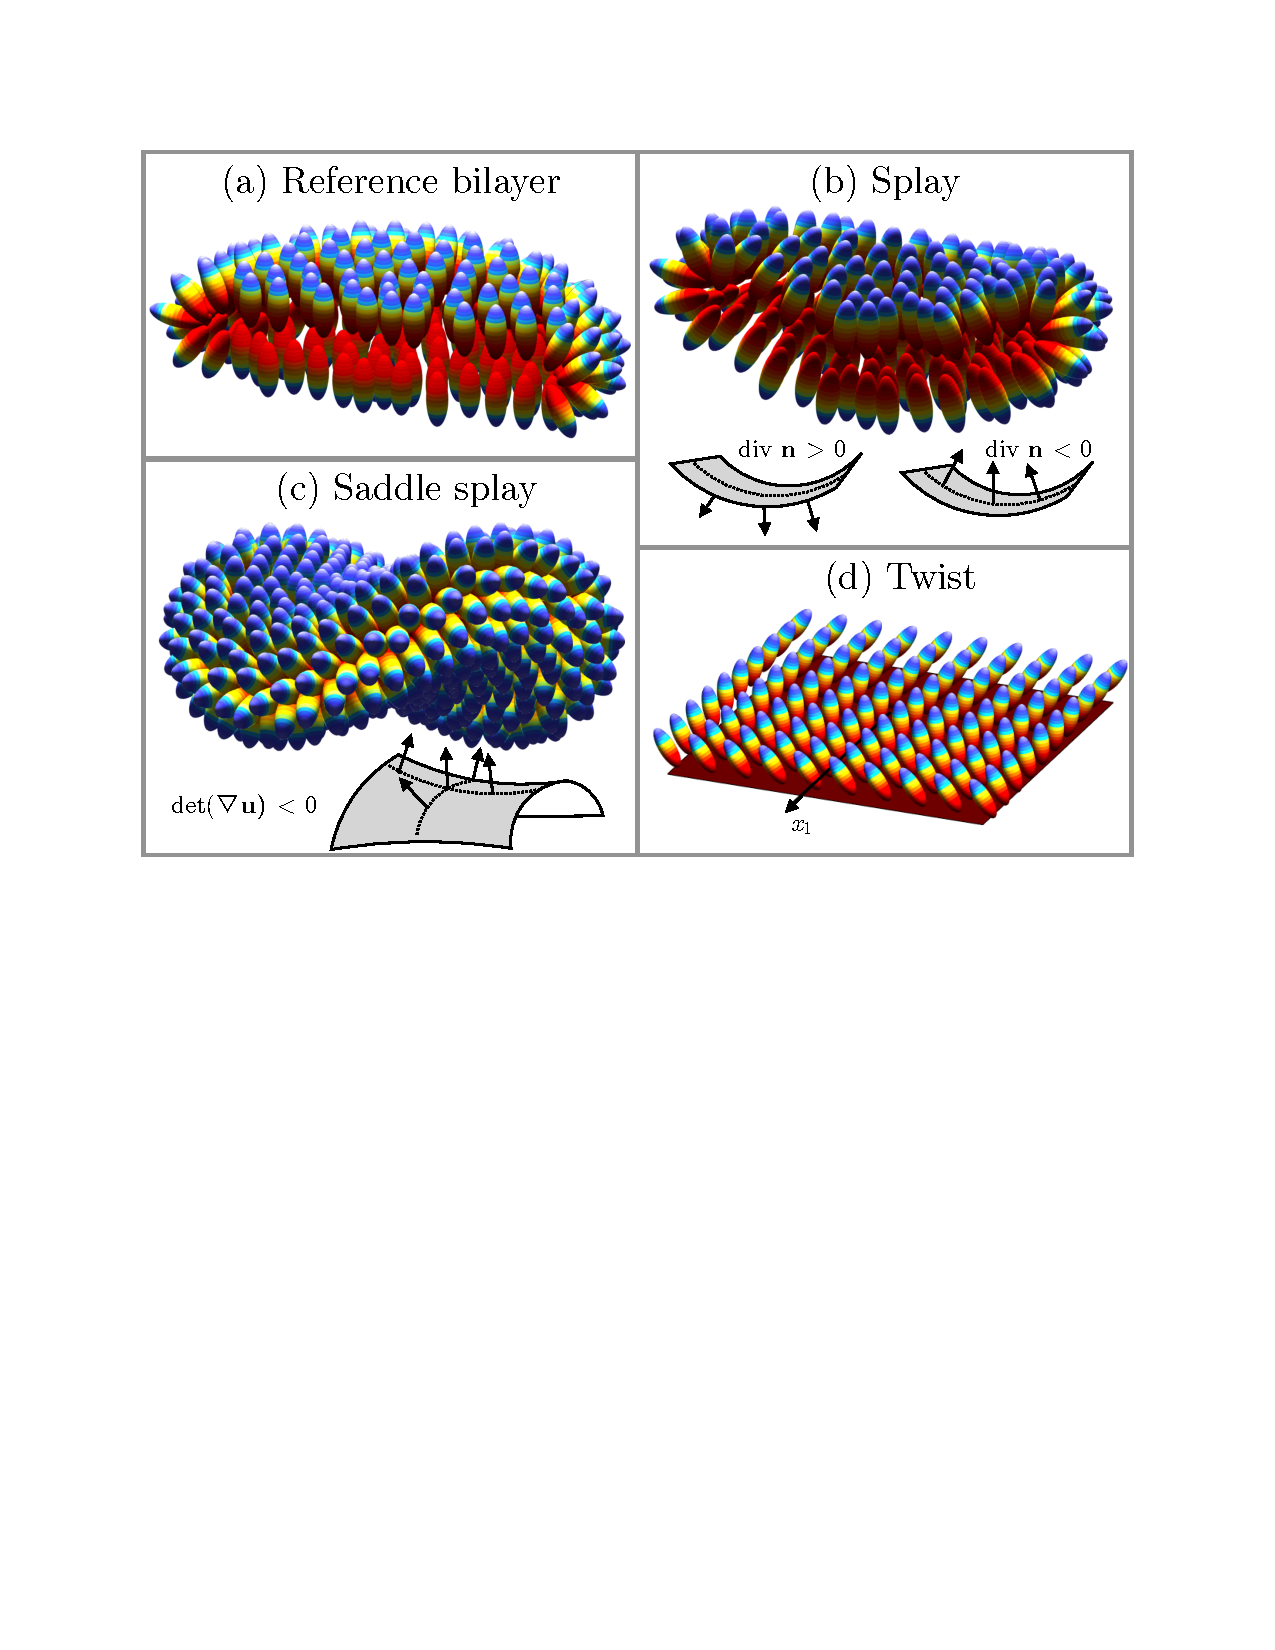
\includegraphics[width=0.80\textwidth]{Figures/Deformations.pdf}}
\vspace{-0.2cm}
\caption{\label{fig:flattening}Example of computing bending modulus of a lipid bilayer from particle simulation.
    }
\end{wrapfigure}
it relaxes from an initially non-equilibrium configuration \cite{PhysRevLett.117.188102}.
Figure~\ref{fig:flattening} shows an example where the initial configuration of a lipid bilayer patch contains only
splay deformation without any other components (saddle splay, twist and tilt). 
As the bent membrane flattens we find that both the membrane self-interaction energy $\Phi$ and the elastic energy ${\cal W}$ decrease,
and because the saddle splay, twist and tilt stay zeros, the slope gives the bending modulus in this case. 


%To characterize material properties of a bilayer, we compare the energies and forces generated by
%a collection of amphiphilic particles against the energies and forces of a continuum bilayer.
%We propose to first {\bf (i)} Assess whether the continuum energies \eqref{ansatz3} are the same
%as the corresponding energies in the particle system for all reasonable deformation.
%If this is the case we will {\bf (ii)} determine the value of the elastic $\KB$,
%$\KT$, $\KG$ and $\KTH$, and then {\bf (iii)} understand how the model parameters $\rho,$ $\gamma$, and particle shape map onto elastic moduli. 
%%
%%Motivated by our preliminary results \cite{Fu2018_SIAM}
%%we use realistic values for particle diameter $2$ nm \cite{Boal},
%%screening length $\rho = 2.5$ nm \cite{Eriksson1989,Lin2005,Parsegian,Israelachvili80,TerziDeserno17}
%%and interfacial tension $\gamma=4.1$ pN nm$^{-1}$ \cite{GarciaSaez, KUZMIN2005, Petelska2012, Jackson}
%%model parameters. The repulsion strength, repulsion length scale, particle shape (e.g. disks, ellipses), 
%%particle diameter and the hydrophobic boundary condition \eqref{SL}
%%are additional parameters defining the coarse-grained representation. 
%
%An accurate and robust way to measure material properties is to track the evolution of the bilayer. 

Here we start with a particle-based bilayer in a specific non-equilibrium shape that consists of only one component of the displacement in figure~\ref{fig:deformations}, 
and then evolve the particle system
%bilayer by steepest gradient descent 
with respect to the HARP functional:
\begin{equation}
\label{SGD}   
\frac{\dif {\bf a}_i}{\dif t} = {\bf F}_i,    \quad  \frac{\dif {\bf R}_i}{\dif t}  = {\bf R}_i A({\bf w}_i),\quad i = 1, \dots, N.
\end{equation}
where that particle centers ${\bf a}_i$ and rotation matrices ${\bf R}_i$ determine the particle configuraton; 
$A({\bf w}_i)$ is the skew-symmetric matrix with axial vector ${\bf w}_i$.
%We solve \eqref{SGD} numerically  using an Adams–Bashforth linear multistep method. 
The procedure involves solving \eqref{SL} based off of the current particle configuration.
We then use the solution $u$ to calculate the collection of forces and torques \eqref{forceandtorque}, and update the particle configuration
through \eqref{SGD}.

\begin{wrapfigure}[12]{l}{0.32\textwidth}
\centerline{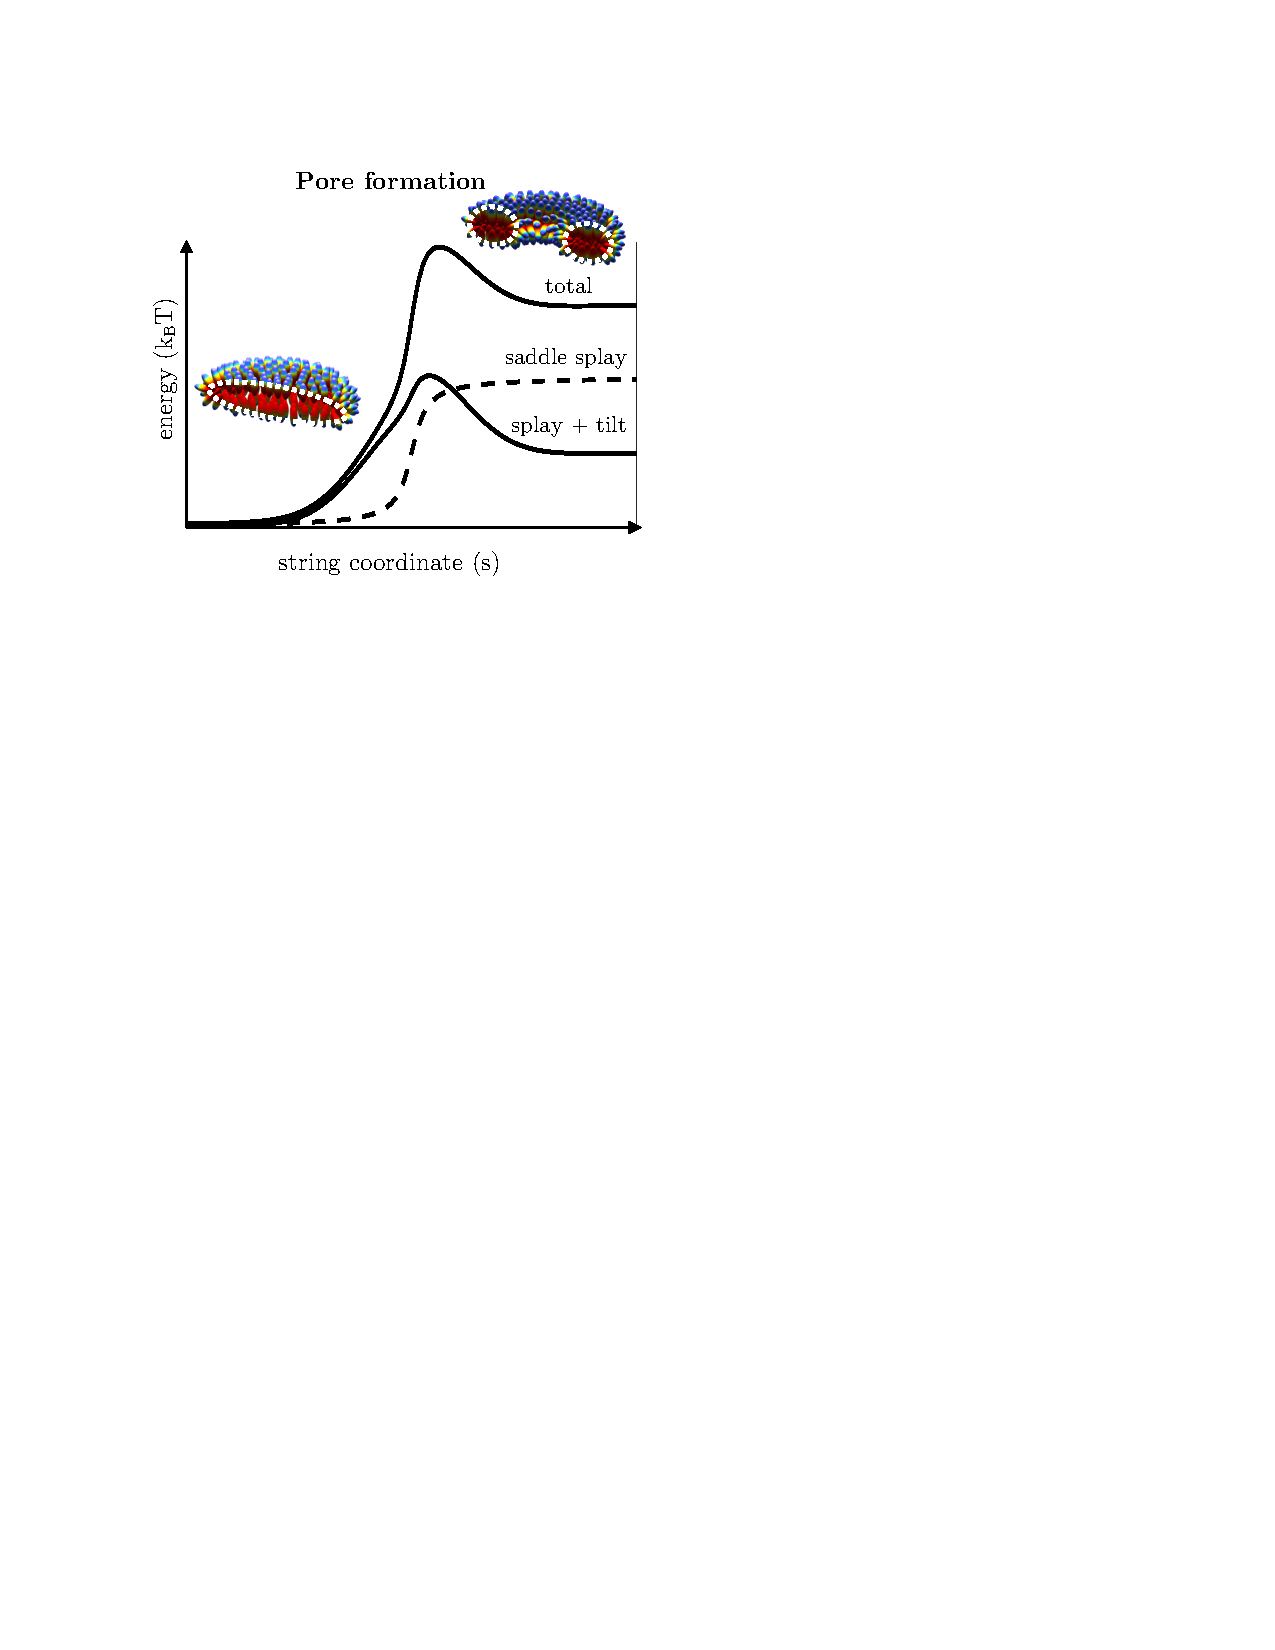
\includegraphics[width=0.32\textwidth]{Figures/SaddleSplayDiagram.pdf}}
\caption{
\label{fig:saddle_splay}  
Determination of saddle splay modulus.
}
\end{wrapfigure}
%
The evolution \eqref{SGD} satisfies the energy dissipation law $\frac{\dif }{\dif t} \Phi \leq 0$
and this stabilizes the evolving bilayer shape.
Therefore, we reconstruct an evolving monolayer dividing surface $\Sigma$ and director field ${\bf n}$ by
interpolating the particle centers and orientations. Using \eqref{ansatz3}, we calculate a continuum energy $E$ from the interpolated shapes.

%In certain instances, the bilayer evolution involves only one or a few of the four fundamental deformations.
%When this occurs, the elastic moduli derive from the coefficients of the linear regression between the HAP energy $\Delta \Phi = \Phi - \Phi_0$
%and continuum energies and $\Delta E = E - E_0$, where  $\Phi_0$ and $E_0$ are respective equilibrium values.

%
%Since it is a particle-based method, the HAP model has a number of advantages over continuum-based descriptions.
%The elastic energy \eqref{ansatz3} couples director gradients to surface geometry through
%the tilt vector field.  Furthermore, bilayer energy is the sum of two monolayer
%energies and the distance between these monolayers varies according to \eqref{LMdeformation}.
%Effects like tilt and varying monolayer thickness appear at lipid domain boundaries, the edge of nanopores and at the boundary of membrane inclusions \cite{PhysRevE.102.042406}.
%These effects are present in the proposed formulation, and the particle-based bilayers can break open and join monolayer-wise 
%as required by fussion and fission. 
%
%Bending is the energetically most consequential deformations. To measure a bending modulus,  
%we deform the midplane of a planar bilayer into the shape of a circular arc.
%This arc stores bending energy in the form of splay $\Div {\bf n}$, while twist, saddle-splay and tilt deformations are zero.
%The splay in the two leaflets approximately cancel when added, making the contribution of spontaneous curvature negligible.
%In the case of a rectangular bialyer, the corresponding elastic energy 
%$E = \int_{\Sigma} \KB \kappa^2$ where $\kappa$ is the curvature of the curved cross-section $C$.
%Figure \ref{} shows the approximately linear relationship between $\Delta \Phi$ and $\Delta E$
%used to values for infer $\KB$. 

We propose to conduct calculations similar to the example of figure~\ref{fig:flattening} for other elastic moduli such as the effective saddle splay modulus $\KG$:
%for a wide range of particle parameters and physical parameters in HARP to 
%
%We will also determine the effective saddle splay modulus $\KG$. 
The gradient descent technique is ineffective for measuring $\KG$ because
the saddle splay energy is largely invariant under shape changes.
In the simplified Canham-Helfrich formulation, saddle splay energy is an indicator of topological transitions, thanks to the  Gauss-Bonnet theorem
\cite{TerziDeserno17}.
PI-RR showed that saddle splay acts as a topological indicator even in the presence of nonzero tilt \cite{RyKlYaCo16}. 

To evaluate $\KG$, we will combine the string method from PI-Ryham's work on fusion \cite{RyKlYaCo16} with
the present particle simulations. 
%The string method is a numerical scheme that finds
%least energy pathways separating energy basins \cite{doi:10.1063/1.2720838}.
%Using the string method, we will evaluate the transition energies between the intact pancake shape,
%and one with a pore. Pore formation in a single bilayer decreases the integral of saddle splay from $4\pi$
%to $0$. We can, in principle, detect this drop in energy because we have already accounted for the other deformations. 
%
%%We will also analyze $\KG$ using a helical geometry. In a helicoid with inclination $m$, the director
%%gradient is $\nabla n = \begin{pmatrix} 0 & m(m^2+x_1^2)^{-1} \\ m(m^2+x_1^2)^{-1} & 0\end{pmatrix}$ where $x_1$ is the distance to the central
%%axis. We observe that saddle splay, twist and tilt are zeros, and $\det \nabla n = m^2(m^2+x_1^2)^{-2}$.
%%In the simulations, the particles forming the helicoid will be confined to two, concentric cylinders. The
%%continuum energy $\tfrac{1}{2}\KG h(m x_1(m^2+x_1^2)^{-1} + \tan^{-1}(x_1/m)) |_{r_1}^{r_2}$ where $h$, $r_1$ and $r_2$
%%are the cylinder heights, inner cylinder radius, and outer cylinder radius, respectively. 
%
The twist deformation is a fully three-dimensional deformation. 
(Specific Aim 3 address outstanding implementation issues like three-dimensional boundary integral solvers.) 
It is closely related to the assumption of lateral fluidity in membranes \cite{Hamm2000}. Note that tilt is locally non-zero whenever twist is non-zero.
That is because the surface gradient $\nabla {\bf n}$ equals the second fundamental form, and is therefore symmetric, whenever ${\bf n} = {\bf N}$ locally. 

%The proposed particle-based simulations of the HARP model in equations~\ref{SGD} also allow direct examination on the assumption of quadratic form of the elastic energy density.
%As discussed earlier, recent disagreement in elastic moduli between continuum model and MD simulations originates from such assumption. 
%The particle-based HARP model provides a unique opportunity to examine the validity of the quadratic elastic energy, and the PIs propose to examine how (if) any deviation from the quadratic elastic energy may depend on the microscopic details of the amphiphilic particles and their interactions.

\subsubsection{HK elastic energy form}
It may come as a surprise then that the field of membrane continuum mechanics still lacks consensus as to
 whether \eqref{ansatz3} contains a complete list of consistent deformations.
\textbf{(i)} Researcher have assumed that $\KT = 0$ \cite{Hamm2000, TerziDeserno17, C9SM02079A, PhysRevE.102.042406}.
  Based on \eqref{eq:twist_energy}, a value $\KT = 0$ leads to the
  unphysical conclusion that there are bilayers with $\nabla {\bf n} \to \infty$ but $E \to 0.$ 
  \textbf{(ii)}
  Recently, \cite{TerziDeserno17} derived a tilt curvature term that was neglected from the HK analysis \cite{Hamm2000}.
  Later, \cite{C9SM02079A} 
  and \cite{PhysRevE.102.042406} independently identified an inconsistency \cite{TerziDeserno17} arising
  from a transversal tilt invariance assumption.
  The PI Ryham showed,  that the tilt vector $T = {\bf n}/{\bf n}\cdot {\bf N} - {\bf N}$ leads to unphysical cusps when constraining membrane thickness  \cite{RyKlYaCo16}.  
  \textbf{(iii)}
  Theoretical analysis of lipid phase transitions predict a negative saddle-splay modulus around $-8$ \kBT\;
\cite{SIEGEL2004366,SIEGEL20085200}. Researchers point out, however, that this theoretical value requires a larger energy 
barrier for monolayer fusion than is found by experiment \cite{FrRoPi17,Tran7106,TerziDeserno17}.
Furthermore, the stability requirements of \eqref{ansatz3} are $\KB > 0$, $K_T > 0$, $\KG \geq -4\KB$
and $\KG \geq -4\KT$. Molecular dynamics investigations find a twist modulus about 1 \kBT \cite{LeVeWa14},
suggesting a somewhat smaller magnitude for $\KG$.

% The form of the elastic energy density \eqref{ansatz3} is the same as
%the Oseen-Frank energy density for nematic liquid crystals \cite{ANDRIENKO2018520,Tran7106,Helfrich73}.   In fact,  
%a lipid monolayer acts as one layer in a smectic  phase \cite{REYESMATEO1995978,Rangamani20140463,PhysRevLett.113.248102}. 
%The constants $\KB$, $\KT$  and $\KG$ play the same role as the Frank constants $K_1$, $K_2$ and $K_{24}$
%liquid crystal theory. However, the ``bend'' distortion from nematics  
%is not present in monolayers since the directors have no dependence in the normal direction.
%There is also no ``spontaneous twist'' in monolayers due to invariance under mirror reflection. 
  
  We suspect the reason why, after twenty years, the field has yet to reach a consensus 
  as to the form of \eqref{ansatz3} has to do with the Taylor expansions used to derive the elastic energy density. 
  Past researchers expressed the strain tensor in
  terms of the orthonormal frame $\{{\bf e}_1, {\bf e}_2, {\bf N}\}$ with surface tangent vectors ${\bf e}_i$ and surface normal ${\bf N}$.  
  In this frame, there is a coupling between the gradients of all three terms ${\bf x}_0,$ $\zeta$ and ${\bf n}$ of the surface deformation field.
  %\eqref{LMdeformation}.
  Subtle differential geometric arguments are needed to evaluate the terms in the Taylor expansion,
  and these couplings can lead to an energy density with more than ten parameters, for example \cite{PhysRevE.102.042406}.
  
  We will revisit the HK analysis to see if any of the aforementioned inconsistencies can be resolved.
  As a main analytical innovation, we have found that expanding the strain tensor in
  terms of the orthonormal frame $\{{\bf e}'_1, {\bf e}'_2, n\}$ with ${\bf e}'_i$ perpendicular to ${\bf n}$
  greatly simplifies the expansion because it decouples the gradient terms. As an illustration, the prominent works
  \cite{TerziDeserno17, PhysRevE.102.042406, Hamm2000, C9SM02079A} utilize an
  incompressibility condition for the lipid elongation function $\zeta$ from \eqref{LMdeformation} that is only approximately true. 
  However, we prove that when expressed in the $\{{\bf e}'_1, {\bf e}'_2, n\}$ frame, the incompressility condition is \emph{exact}
  and is given by a Steiner-type polynomial in terms of $\Div {\bf n}$ and $\det \nabla {\bf n}$ \cite{Fe59}.
  Aside from the special case of zero tilt, \cite{Hamm2000} and coworkers seem to have been unaware of this result.

%To measure the twist modulus, we place a single monolayer on a hydrophobic substrate 
%and take the initial configuration ${\bf n} = (0, f(x_1), \sqrt{1 - f^2(x_1)})$,
%yielding a surface gradient $\nabla {\bf n} = \begin{pmatrix}0 & 0\\ f'(x_1) & 0\end{pmatrix}$. 
%  Here $\Div {\bf n} = \mathrm{tr}(\nabla {\bf n}) = 0$, $\det(\nabla {\bf n}) = 0$ and
%  $\Curl {\bf n} = (\nabla u)_{12} - (\nabla u)_{21} = f'(x_1)$.
%  This gives the continuum elastic energy equals
%  \begin{equation}
%    \label{eq:twist_energy}
%    E = \int_{\Sigma} \tfrac{1}{2}\KT (f'(x_1))^2 + \tfrac{1}{2} \KTH f^2(x_1) \,\dif dx_1 \dif x_2,
%  \end{equation}
%  which we compare to the HAP simulation data.

%\subsubsection{Asymptotic analysis on the limit $\rho\rightarrow 0$}
%The HAP energy converges to the surface energy in the limit of vanishing screening length 
%and the boundary layers of the minimizers (the solutions to the screen Laplace equation) converges to 
%area measures supported on the particle boundaries.  This is analogous to the sharp interface limit in the phase-field functional formulation \cite{Modica87, MODICA1987487, LuMo89}. 
%PI RR has worked directly on phase field approximations of membrane bending energy 
%\cite{0951-7715-18-3-016} and asymptotcs in the Poisson-Boltzman equation \cite{1531-3492_2006_2_357,Lee2018}.
%The proposed analysis is a natural outgrowth or prior work because the linearization of the Poisson-Boltzmann equation is the screened Laplace equations \eqref{SL}.
%
%We will develop some of the mathematical connections between the HAP energy and the energy functionals used in the gradient theory of phase transitions. 
%%The phase field functional approximates the perimeter of sublevel sets of a so-called phase field indicator function. 
%%The approximation becomes sharp in the zero interfacial thickness limit and minimizers of the phase field functional converge (after normalization) 
%%to the characteristic function of a set solving a perimeter minimization problem 
%%\cite{Modica87, MODICA1987487, LuMo89}. 
%%
%%
%One of the basic questions is to establish the HAP convergence rate as a function of particle geometry 
%\cite{LuMo89}, which can be used as an essential benchmark for numerical validation. 
%In the context of microstructure fabrication, the particle configurations maximally sequester hydrophobic surfaces.  
%As an illustration, consider two fluid-bound plates $P_1$ and $P_2$ that geometrically flat and hydrophobic all sides.
%We conjecture that in the zero-screening length limit, the plates have overlapping faces, and that 
%\begin{equation}
%\lim_{\rho \to 0} \min \Phi_{\text{hydro}} = \max_{\mathcal{X}} A(P_1 \Delta P_2)
%\end{equation}
%$A(P_1 \Delta P_2)$ is the area of the symmetric difference of the overlap.  
%\cite{https://doi.org/10.1038/s41467-019-09787-6}


% It may come as a surprise then that the field of membrane continuum mechanics still lacks consensus as to
% whether \eqref{ansatz3} contains a complete list of consistent deformations.
%\textbf{(i)} Researcher have assumed that $\KT = 0$ \cite{Hamm2000, TerziDeserno17, C9SM02079A, PhysRevE.102.042406}.
%  Based on \eqref{eq:twist_energy}, a value $\KT = 0$ leads to the
%  unphysical conclusion that there are bilayers with $\nabla {\bf n} \to \infty$ but $E \to 0.$ 
%  \textbf{(ii)}
%  Recently, \cite{TerziDeserno17} derived a tilt curvature term that was neglected from the HK analysis \cite{Hamm2000}.
%  Later, \cite{C9SM02079A} 
%  and \cite{PhysRevE.102.042406} independently identified an inconsistency \cite{TerziDeserno17} arising
%  from a transversal tilt invariance assumption.
%  The PI Ryham showed,  that the tilt vector $T = {\bf n}/{\bf n}\cdot {\bf N} - {\bf N}$ leads to unphysical cusps when constraining membrane thickness  \cite{RyKlYaCo16}.  
%  \textbf{(iii)}
%  Theoretical analysis of lipid phase transitions predict a negative saddle-splay modulus around $-8$ \kBT\;
%\cite{SIEGEL2004366,SIEGEL20085200}. Researchers point out, however, that this theoretical value requires a larger energy 
%barrier for monolayer fusion than is found by experiment \cite{FrRoPi17,Tran7106,TerziDeserno17}.
%Furthermore, the stability requirements of \eqref{ansatz3} are $\KB > 0$, $K_T > 0$, $\KG \geq -4\KB$
%and $\KG \geq -4\KT$. Molecular dynamics investigations find a twist modulus about 1 \kBT \cite{LeVeWa14},
%suggesting a somewhat smaller magnitude for $\KG$.

 
%The form of the elastic energy density \eqref{ansatz3} is the same as
%the Oseen-Frank energy density for nematic liquid crystals \cite{ANDRIENKO2018520,Tran7106,Helfrich73}.   In fact,  
%a lipid monolayer acts as one layer in a smectic  phase \cite{REYESMATEO1995978,Rangamani20140463,PhysRevLett.113.248102}. 
%The constants $\KB$, $\KT$  and $\KG$ play the same role as the Frank constants $K_1$, $K_2$ and $K_{24}$
%liquid crystal theory. However, the ``bend'' distortion from nematics  
%is not present in monolayers since the directors have no dependence in the normal direction.
%There is also no ``spontaneous twist'' in monolayers due to invariance under mirror reflection. 
%  
%  We suspect the reason why, after twenty years, the field has yet to reach a consensus 
%  as to the form of \eqref{ansatz3} has to do with the Taylor expansions used to derive the elastic energy density. 
%  Past researchers expressed the strain tensor in
%  terms of the orthonormal frame $\{{\bf e}_1, {\bf e}_2, {\bf N}\}$ with surface tangent vectors ${\bf e}_i$ and surface normal ${\bf N}$.  
%  In this frame, there is a coupling between the gradients of all three terms ${\bf x}_0,$ $\zeta$ and ${\bf n}$ of the deformation \eqref{LMdeformation}.
%  Subtle differential geometric arguments are needed to evaluate the terms in the Taylor expansion,
%  and these couplings can lead to an energy density with more than ten parameters, for example \cite{PhysRevE.102.042406}.
%
%  We will revisit the HK analysis to see if any of the aforementioned inconsistencies can be resolved.
%  As a main analytical innovation, we have found that expanding the strain tensor in
%  terms of the orthonormal frame $\{{\bf e}'_1, {\bf e}'_2, n\}$ with ${\bf e}'_i$ perpendicular to ${\bf n}$
%  greatly simplifies the expansion because it decouples the gradient terms. As an illustration, the prominent works
%  \cite{TerziDeserno17, PhysRevE.102.042406, Hamm2000, C9SM02079A} utilize an
%  incompressibility condition for the lipid elongation function $\zeta$ from \eqref{LMdeformation} that is only approximately true. 
%  However, we prove that when expressed in the $\{{\bf e}'_1, {\bf e}'_2, n\}$ frame, the incompressility condition is \emph{exact}
%  and is given by a Steiner-type polynomial in terms of $\Div {\bf n}$ and $\det \nabla {\bf n}$ \cite{Fe59}.
%  Aside from the special case of zero tilt, \cite{Hamm2000} and coworkers seem to have been unaware of this result.

Our investigations will leave open the possibility that the free energy of monolayers and bilayers is non-local. 
We have shown that hydrophic attraction is a non-additive force, meaning the force of attraction between two
particles is dependent on the position a third or more particles \cite{SilveraBatista1242477}.
Conceptually, this would arise in continuum theory if two monolayer surfaces
had a different elastic energy density despite having locally identical curvatures and directors.
The boundary integral formulation described in Specific Aim 3 easily accomodates additional linear PDE and
we will extend our study to include charge lipids and weak electrolytes \cite{C9SM00772E}.



